\documentclass{article}
\usepackage{tikz}
\usepackage{graphicx}
\usepackage{amsmath,amssymb}
\usepackage{hyperref}
\hypersetup{ colorlinks=true, linkcolor=blue }
\title{Moment of Inertia}

\begin{document}
\maketitle
\tableofcontents

\section{Intro}
\subsection{Definition}
Moment of Inertia is denoted by the letter 'I' and is the product of the mass times the square of the radius of gyration.
$$ I = M R^2$$
\subsection{Parallel Axis Theorem}
Moment of inertia of an object about an axis parallel to another axis is related by the parallel axis theorem.\\
Let I be the moment of inertia about an axis,\\
I' be the moment of Inertia about an axis parallel to it,\\
$x$ be the distance between those axis,\\
$M$ be the mass of object. Then
$$I' = I + M x^2$$

\subsection{Perpendicular Axis Theorem}
For a planar object, the moment of inertia about an axis perpendicular to the plane is the sum of the moments of inertia of two perpendicular axes through the same point in the plane of the object.
$$ I_z = I_x + I_y$$
where $I_x$,$I_y$ are the moment of inertia about axis in the plane of the object and $I_z$ is the moment of inertia about an axis perpendicular to the plane of the object.

\section{Uniform Rod}
\subsection{Axis passing through its midpoint}
\begin{tikzpicture}
  \draw (0,0) rectangle (6,0.5);
  \draw[dashed] (3,1) -- (3,-0.5);
  \draw (3,-1) node {$x$=0};
\end{tikzpicture}
\\
Consider a uniform rod of length L and mass M rotating about an axis passing through the centre of gravity and perpendicular to the rod.
Let us consider a small element with mass $dm$ and length $dx$ at a distance $x$ from the axis. Then,
$$I = \int dm*x^2$$
$$dm = \frac{M}{L} dx$$
$$\therefore I = \int_{-\frac{L}{2}}^{\frac{L}{2}} \frac{M}{L} x^2 dx$$
$$ I = \frac{M}{L} \left[ \frac{x^3}{3} \right]_{\frac{-L}{2}}^{\frac{L}{2}}$$
$$ I = \frac{M}{3L} \left[ \frac{L^3}{8} - \left(-\frac{L^3}{8}\right) \right]$$
$$ I = \frac{M}{3L} \left[ \frac{L^3}{8} + \frac{L^3}{8} \right]$$
$$ \boxed{I = \frac{ML^2}{12}} $$

\subsection{Axis passing through its end}
\begin{tikzpicture}
  \draw (0,0) rectangle (6,0.5);
  \draw[dashed] (0,1) -- (0,-0.5);
  \draw (0,-1) node {$x$=0};
\end{tikzpicture}
\\
Consider a uniform rod of length L and mass M rotating about an axis passing through one end of the rod.
Let us consider a small element with mass $dm$ and length $dx$ at a distance $x$ from the axis. Then,
$$I = \int dm*x^2$$
$$dm = \frac{M}{L} dx$$
$$\therefore I = \int_{0}^{L} \frac{M}{L} x^2 dx$$
$$ I = \frac{M}{L} \left[ \frac{x^3}{3} \right]_{0}^{L}$$
$$ I = \frac{M}{3L} \left[ 0 - \left( -L^3\right) \right]$$
$$ I = \frac{M}{3L} \left[ L^3 \right]$$
$$ \boxed{I = \frac{ML^2}{3}} $$

\section{Ring}
\subsection{Axis through centre and perpendicular to the plane of the ring}
\begin{figure}[h!]
  \centering
  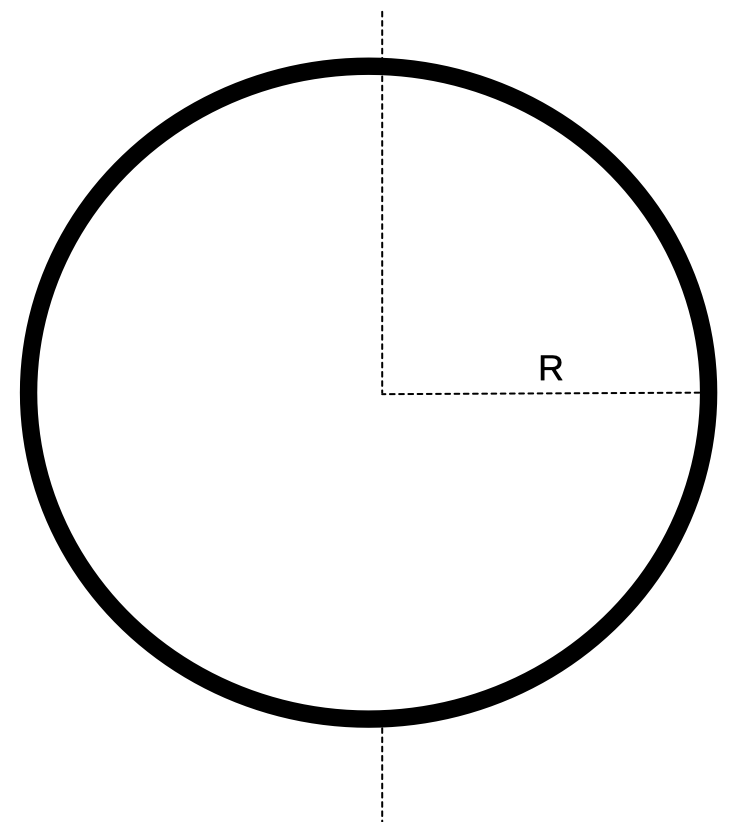
\includegraphics[scale=0.3]{ring1.png}
\end{figure}
Consider a uniform ring of radius R and mass M rotating about an axis passing through the centre of gravity and perpendicular to the plane of the ring.
Let us consider a small element with mass $dm$ and length $Rd\theta$
$$dm = \frac{M}{2\pi R} Rd\theta$$
$$I = dm R^2$$
$$I = \int_{0}^{2\pi} \frac{M}{2\pi} R^2 d\theta$$
$$\boxed{I = MR^2}$$

\subsection{About the diameter}
\begin{figure}[h!]
  \centering
  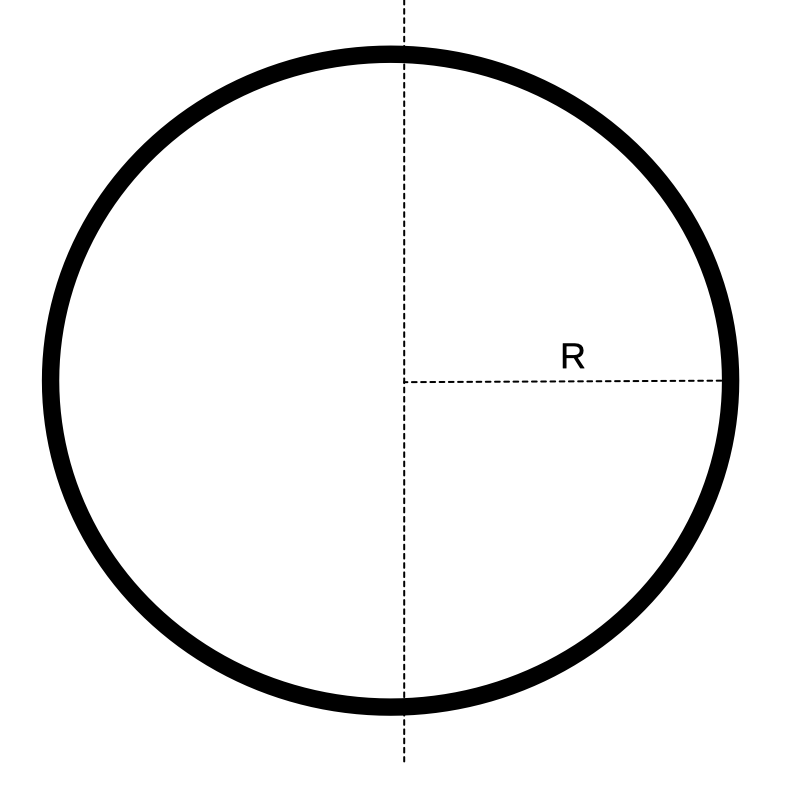
\includegraphics[scale=0.3]{ring2.png}
\end{figure}
The moment of inertia about axis through the centre and perpendicular to the plane of ring is $MR^2$. Moment of inertia about diameter in the plane of the ring is I.\\
$\therefore$ Using perpendicular axis theorem,
$$MR^2 = 2I$$
$$\boxed{I = \frac{MR^2}{2}}$$

\section{Disk}
\subsection{Axis through the centre and perpendicular to the plane of the disk}
\begin{figure}[h!]
  \centering
  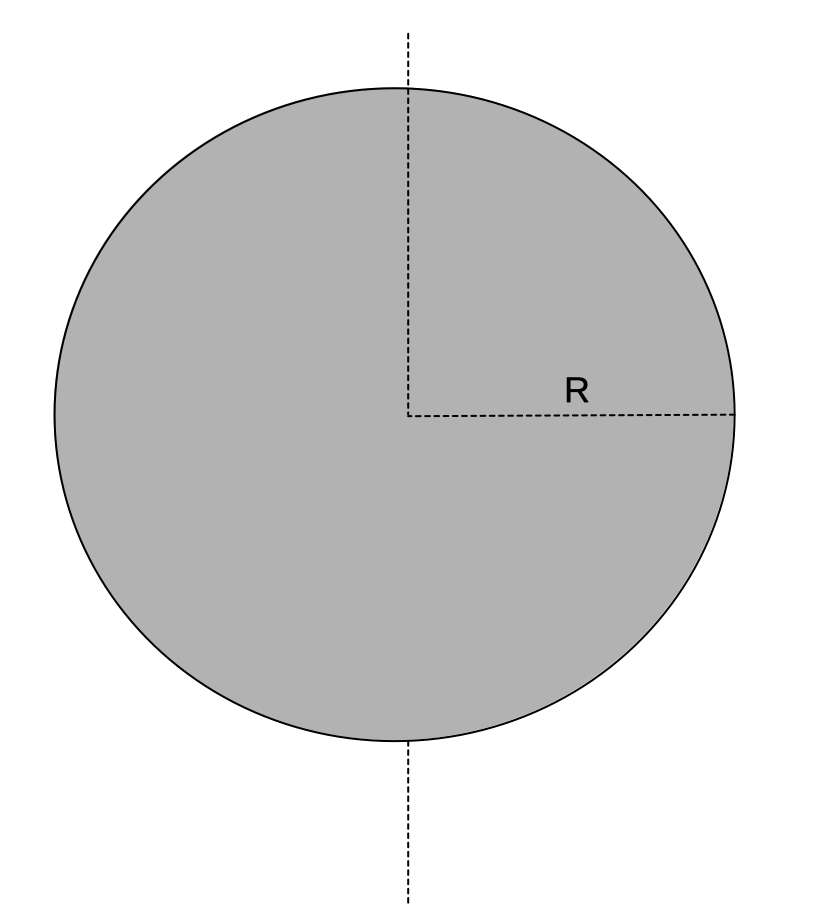
\includegraphics[scale=0.3]{disk1.png}
\end{figure}
Cosider a uniform disk of radius R and mass M rotating about an axis passing through the centre of gravity and perpendicular to the plane of the disk.
Let us consider a ring of radius with mass $dm$ and radius $x$ and thickness $dx$
$$dm = \frac{M}{\pi R^2} 2\pi x dx$$
$$dI = dm x^2$$
$$I = \int_{0}^{R} \frac{M}{R^2} 2 x^3 dx$$
$$I = \frac{2M}{R^2} \left[ \frac{x^4}{4} \right]_{0}^{R}$$
$$\boxed{I = \frac{MR^2}{2}}$$

\subsection{About the diameter}
\begin{figure}[h!]
  \centering
  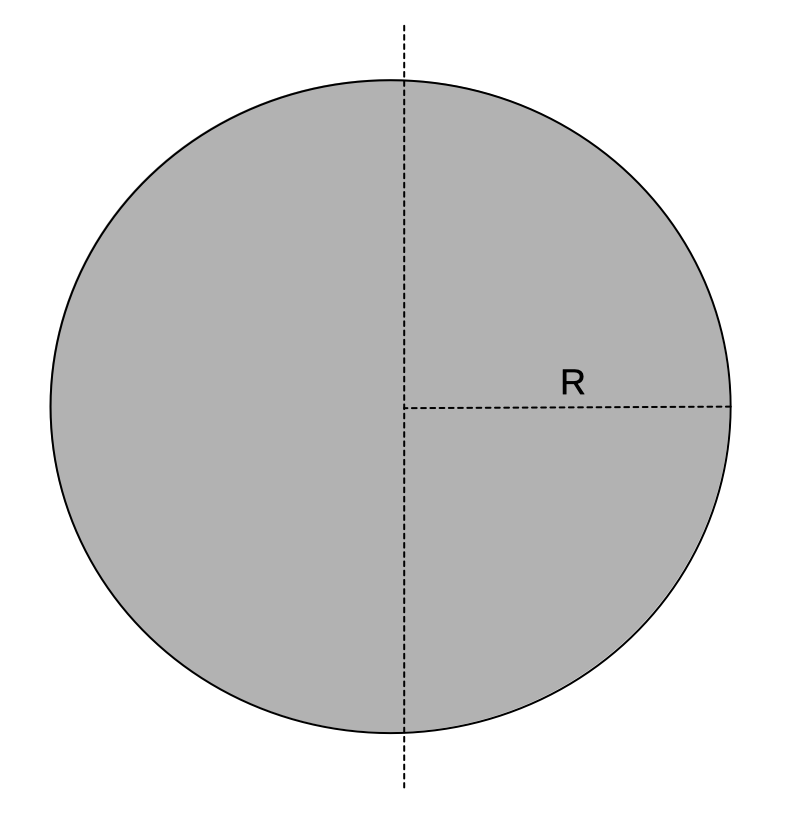
\includegraphics[scale=0.3]{disk2.png}
\end{figure}
The moment of inertia about axis through the centre and perpendicular to the plane of ring is $\frac{MR^2}{2}$. Moment of inertia about diameter in the plane of the ring is I.\\
$\therefore$ Using perpendicular axis theorem,
$$\frac{MR^2}{2} = 2I$$
$$\boxed{I = \frac{MR^2}{4}}$$

\section{Hollow Cylinder}
\subsection{Axis through its centre and perpendicular to the circular faces}
Consider a hollow cylinder of radius R, height h and mass M rotating about an axis passing through its centre and perpendicular to the circular faces. Let the hollow cylinder be made up of many rings.
Let us consider a ring of mass $dm$ and thickness $dx$
$$dm = \frac{M}{2\pi Rh}2\pi R dx$$
$$dI = dm R^2$$
$$dI = \frac{M}{h} R^2 dx$$
$$I = \int_0^h \frac{MR^2}{h} dx$$
$$\boxed{I = MR^2}$$

\subsection{Axis through its centre and perpendicular to the lateral side}
Consider a hollow cylinder of radius R, height h and mass M rotating about an axis passing through its centre and perpendicular to the lateral side. Let us consider a ring of mass $dm$ and thickness $dx$
$$dm = \frac{M}{2\pi Rh} 2\pi Rdx$$
$$dI = \frac{dmR^2}{2} + dmx^2$$
$$dI = \frac{MR^2}{2h} dx + \frac{Mx^2}{h} dx$$
$$I = \int_{\frac{-h}{2}}^{\frac{h}{2}} \frac{MR^2}{2h} + \frac{Mx^2}{h} dx$$
$$I = \left[ \frac{MR^2}{2h}x + \frac{Mx^3}{3h} \right]_{\frac{-h}{2}}^{\frac{h}{2}}$$
$$\boxed{I = \frac{MR^2}{2} + \frac{Mh^2}{12}}$$

\section{Solid Cylinder}
\subsection{Axis through its centre and perpendicular to the circular faces}
\begin{figure}[h!]
  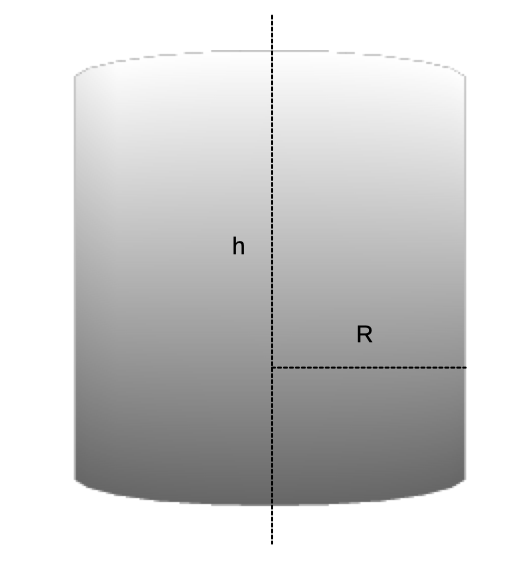
\includegraphics[scale=0.5]{cylinder1.png}
  \centering
\end{figure}
Consider a solid cyclinder of radius R, height h and mass M rotating about an axis passing through its centre and perpendicular to the circular faces. Let the solid cylinder be made up of many hollow cylinder.
Let us consider a hollow cylinder of mass $dm$, thickness $dx$, radius $x$
$$dm = \frac{M}{\pi R^2h}2\pi xdx h$$
$$dI = dmx^2$$
$$dI = 2MR^2x^3dx$$
$$I = \int_0^h 2MR^2x^3 dx$$
$$I = \left[ \frac{MR^2x^4}{2} \right]_0^h$$
$$\boxed{I = \frac{MR^2}{2}}$$

\subsection{Axis through its centre and perpendicular to lateral face}
\begin{figure}[h!]
  \centering
  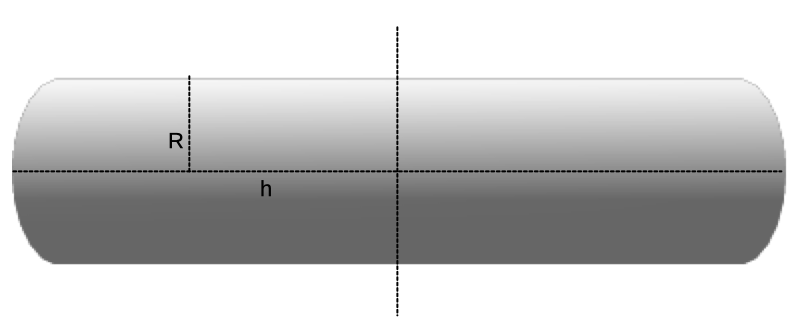
\includegraphics[scale=0.5]{cylinder2.png}
\end{figure}
Consider a solid cyclinder of radius R, height h and mass M rotating about an axis passing through its centre and perpendicular to lateral face. Let the solid cylinder be made up of many hollow cylinders.
Let us consider a hollow cylinder of mass $dm$, height $h$, thickness $dx$ and radius $x$.
$$dm = \frac{M}{\pi R^2 h}2\pi xdxh$$
$$dI = \frac{dmx^2}{2} + \frac{dmh^2}{12}$$
$$dI = \frac{Mx^3}{R^2} dx + \frac{2Mxh^2}{12R^2} dx$$
$$I = \int_0^R \frac{Mx^3}{R^2} + \frac{Mxh^2}{6R^2} dx$$
$$I = \left[ \frac{Mx^4}{4R^2} + \frac{Mx^2h^2}{12R^2} \right]_0^R$$
$$\boxed{I = \frac{MR^2}{4} + \frac{Mh^2}{12}}$$

\section{Spherical Shell}
\subsection{About its centre}
\begin{figure}[h!]
  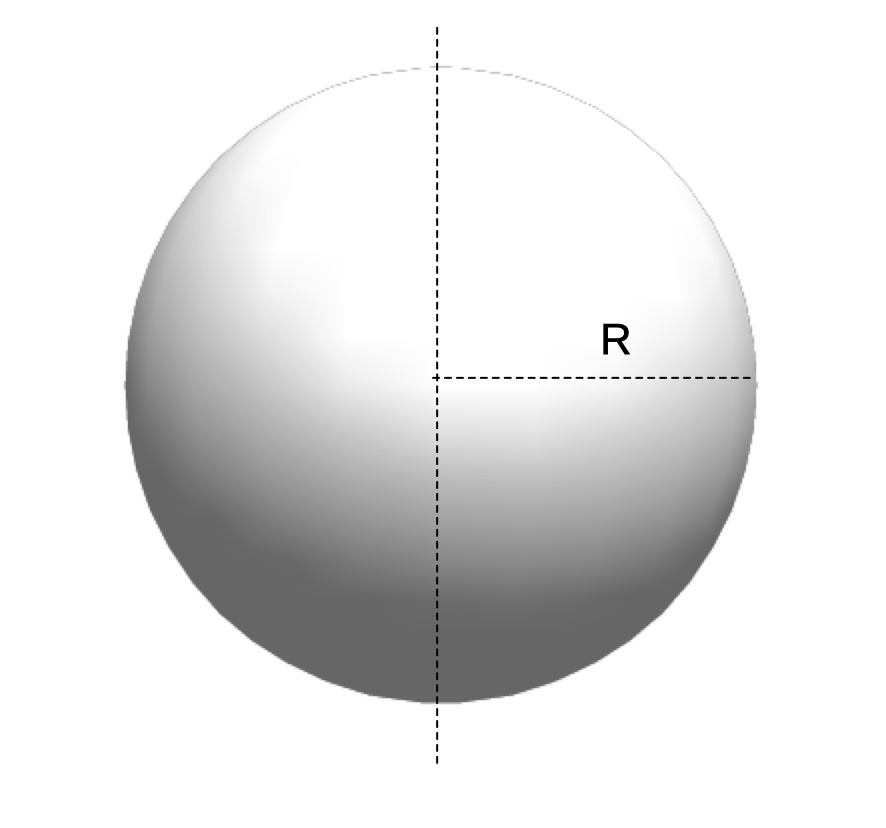
\includegraphics[scale=0.3]{sphere.png}
  \centering
\end{figure}
Consider a spherical shell of radius R and mass M rotating about its centre.
Let us consider it to be made up of many rings of radius $y$ thickness $yd\theta$ and mass $dm$. Also, $$x=R\cos{\theta}$$ $$y=R\sin{\theta}$$
$$dm = \frac{M}{4\pi R^2} 2\pi y Rd\theta$$
$$dI = dmy^2$$
$$dI = \frac{My^3}{2R} d\theta$$
$$I = \int_0^{\pi} \frac{MR^2\sin^3{\theta}}{2} d\theta$$
$$I = \int_0^{\pi} \frac{MR^2\left(3\sin{\theta}-\sin{3\theta}\right)}{8} d\theta$$
$$I = \frac{MR^2}{8} \left[-3\cos(\theta) + \frac{\cos{3\theta}}{3}\right]_0^{\pi}$$
$$I = \frac{MR^2}{8}\left[3-\frac{1}{3}+3-\frac{1}{3}\right]$$
$$I = \frac{MR^2}{8}\frac{16}{3}$$
$$\boxed{I = \frac{2MR^2}{3}}$$

\section{Solid Sphere}
\subsection{About its centre}
\begin{figure}[h!]
  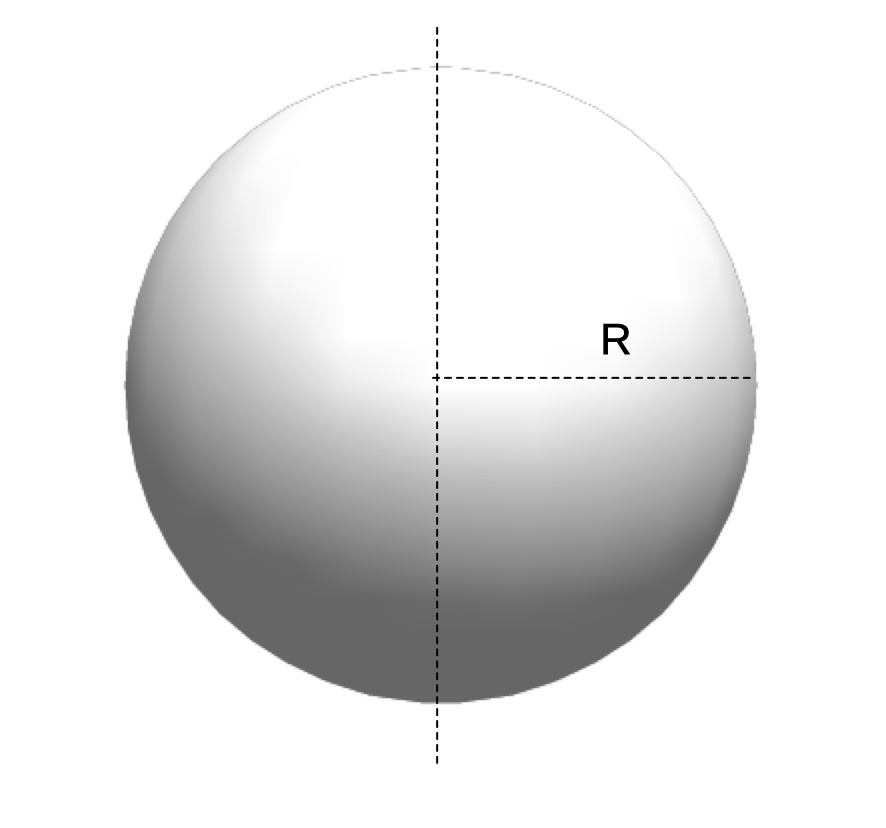
\includegraphics[scale=0.3]{sphere.png}
  \centering
\end{figure}
Consider a solid sphere of radius R and mass M rotating about its centre.
Let us consider it to be made up of many hollow spheres with radius $x$, thickness $dx$ and mass $dm$.
$$dm = \frac{3M}{4\pi R^3} 4\pi x^2 dx$$
$$dI = \frac{2dmx^2}{3}$$
$$dI = \frac{2Mx^4}{R^3} dx$$
$$I = \int_0^R \frac{2Mx^4}{R^3} dx$$
$$\boxed{I = \frac{2MR^2}{5}}$$

\section{Solid Cone}
\subsection{Axis through the centre and perpendicular to the base}
\begin{figure}[h!]
  \centering
  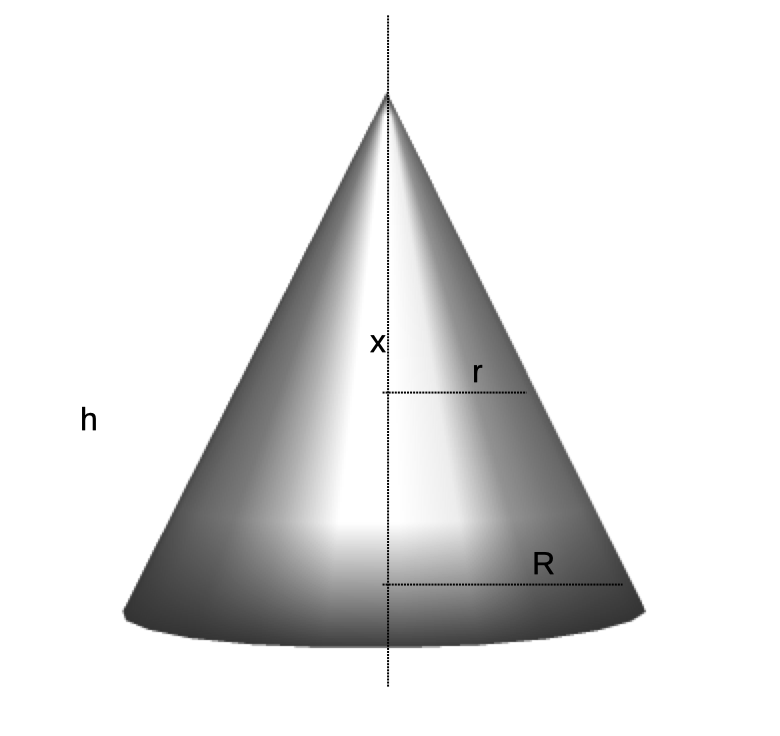
\includegraphics[scale=0.3]{cone1.png}
\end{figure}
Consider a uniform cone of height h, base radius R and mass M rotating about an axis passing through centre of the base and perpendicular to base.
Let us consider it to be made up of many disks of radius $r$, thickness $dx$ and mass $dm$. Also, we have from similarity of triangles
$$\frac{r}{R} = \frac{x}{h}$$
$$dm = \frac{3M}{\pi R^2h} \pi r^2 dx$$
$$dI = \frac{dmr^2}{2}$$
$$dI = \frac{3Mr^4}{2R^2h} dx$$
$$dI = \frac{3MR^4x^4}{2R^2h^5} dx$$
$$I = \int_0^h \frac{3MR^2x^4}{2h^5} dx$$
$$\boxed{I = \frac{3MR^2}{10}}$$

\subsection{Roatating about it tip}
\begin{figure}[h!]
  \centering
  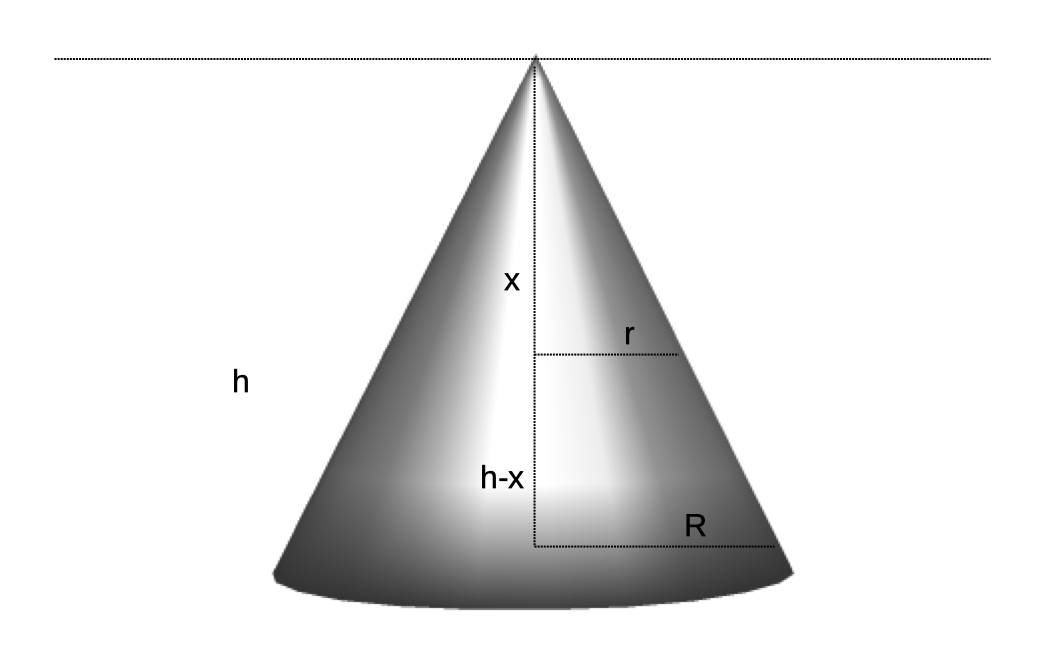
\includegraphics[scale=0.3]{cone2.png}
\end{figure}
Consider a uniform solid cone of height h, base radius R and mass M roatating about an axis passing through its tip. Let us consider it to be made up of disks of radius $r$, thickness $dx$ and mass $dm$. Also, we have from similarity of triangles
$$\frac{r}{R} = \frac{x}{h}$$
$$\implies r = \frac{R}{h}x$$
$$dm = \frac{3M}{\pi R^2h}\pi r^2 dx = \frac{3Mr^2dx}{R^2h}$$
Using parallel axis theorem,\\
Moment of inertia of the small disk about the required axis = Moment of inertia of disk about its diameter + (Mass of the element) $\cdot$ distance from axis
$$dI = \frac{dmr^2}{4} + dmx^2$$
$$dI = \frac{3Mr^4}{4R^2h}dx + \frac{3Mr^2x^2}{R^2h}dx$$
$$dI = \frac{3MR^2x^4}{4h^5}dx + \frac{3Mx^4}{h^3}dx$$
$$I = \int_0^h \frac{3MR^2x^4}{4h^5} + \frac{3Mx^4}{h^3} dx$$
$$I = \left[ \frac{3MR^2x^5}{20h^5} + \frac{3Mx^5}{5h^3} \right]_0^h$$
$$\boxed{I = \frac{3MR^2}{20} + \frac{3Mh^2}{5}}$$

\subsection{Rotating about its base}
\begin{figure}[h!]
  \centering
  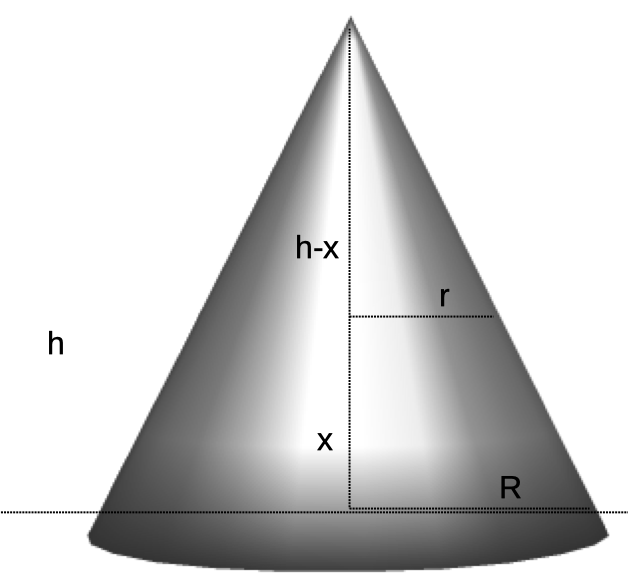
\includegraphics[scale=0.3]{cone3.png}
\end{figure}
Consider a uniform solid cone of height h, base radius R and mass M rotating about an axis along the base diameter. Let us consider it to be made up of many small disks of radius $r$, thickness $dx$ and mass $dm$. Also, we have from similarity of triangles
$$\frac{r}{R} = \frac{h-x}{h}$$
$$\implies r = \frac{R}{h}(h-x)$$
$$dm = \frac{3M}{\pi R^2h}\pi r^2dx = \frac{3Mr^2dx}{R^2h}$$
Using parallel axis theorem,\\
Moment of inertia of the small disk about the required axis = Moment of inertia of disk about its diameter + (Mass of the element) $\cdot$ distance from axis
$$dI = \frac{dmr^2}{4} + dmx^2$$
$$dI = \frac{3Mr^4}{4R^2h} dx + \frac{3Mr^2x^2}{R^2h}x^2$$
$$dI = \frac{3MR^2(h-x)^4}{4h^5} + \frac{3M(h-x)^2x^2}{h^3} dx$$
$$I = \int_0^h \frac{3MR^2(h-x)^4}{4h^5} + \frac{3M(h-x)^2x^2}{h^3} dx$$
$$\boxed{I = \frac{3MR^2}{20} + \frac{Mh^2}{10}}$$
\end{document}
